\documentclass{beamer}

\mode<presentation>
{
  \usetheme{classic}
  \setbeamercovered{transparent}
}

\usepackage[english]{babel}
\usepackage[latin1]{inputenc}
\usepackage{times}
\usepackage[T1]{fontenc}
\usepackage{url}

\title[CLS]{Back to the Future: Life beyond R, by going back to Lisp}
\subtitle{Using History to Design better data analysis systems}
\author[] 
{A.J.~(Tony)~Rossini}

\institute[Novartis Pharma AG and University of Washington]
{
  Quantitative Safety and Epidemiology\\
  Novartis Pharma AG \\
  Basel
  \and
  Department of Biomedical and Health Informatics\\
  University of Washington}

\date[StatComp 2014] % (optional, should be abbreviation of conference name)
{Reisensburg, 2014}
\subject{Statistical Computing Environments}


% Delete this, if you do not want the table of contents to pop up at
% the beginning of each subsection:
\AtBeginSubsection[]
{
  \begin{frame}<beamer>{Outline}
    \tableofcontents[currentsection,currentsubsection]
  \end{frame}
}


\begin{document}

\begin{frame}
  \titlepage
\end{frame}

\begin{frame}[fragile]{Intro to Lisp notation}
\begin{verbatim}
;; This is a comment
#|
    and so is this
|#
'(a list of things to become data)
(list a list of things to become data)
(what-I-execute with-one-thing with-two-thing)
;; that is:
(my-fcn-name input1 
             input2) ; and to auto-gen input1:
(my-fcn-name (my-fcn-name input3 input4)
             input2)
\end{verbatim}
\end{frame}  

\begin{frame}[fragile]{Consider XML}
\begin{verbatim}
<car brand="honda" engine="4cyl">accord</car>
\end{verbatim}
becomes
\begin{verbatim}
; data follows keywords...
(car :brand 'honda :engine "4cyl" 'accord)
\end{verbatim}
\end{frame}


\section{Common Lisp Statistics}
\label{sec:CLS}

\subsection{Why Common Lisp Statistics}
\label{sec:why}

\begin{frame}{What is CLS?}
  \begin{itemize}
  \item A collection of Common Lisp packages
  \item a component-based structure for statistical computing,
    allowing for small and specific specification.
  \item a means to drive philosophically customized data analysis, the
    incorporation of computable statistical research, and the
    enforcement of a structure to allow simple comparisons between
    methodologies.
  \item This is a ``customization'' of a sophisticated programming
    language through packages to support statistical computing, not a
    independent language.  ``Ala Carte'', not ``Menu''.
  \end{itemize}
\end{frame}


\begin{frame}{Current Functionality}
  \begin{itemize}
  \item basic dataframes (similar to R) in 2 different approaches;
    subsetting API under development.
  \item Basic regression (similar to XLispStat)
  \item matrix storage both in foreign and lisp-centric storage
    through lisp-matrix
  \item LAPACK (small percentage implemented, increasing), works
    across both matrix storage types.
  \item static graphics (X11) including preliminary grid functionality
    based on CAIRO.  Generation of PNG files from graphics windows.
    Currently broken due to 3rd party upgrade
  \item CSV file support
  \item Common Lisp!
  \end{itemize}
\end{frame}

\begin{frame}[fragile]{Computational Environment Supported}
  \begin{itemize}
  \item works on Linux, with recent SBCL versions
  \item Definitely works on bleeding edge Debian (unstable).
  \item Has worked for weak definitions of ``work'' on 4 different
    people's computers (not quite, but sort of requires a
    \verb+/home/tony/+ !)
  \end{itemize}
\end{frame}

\begin{frame}{Goals}{short term}
  \begin{itemize}
  \item Better integration of data structures with statistical routines
    (auto-handling with dataframes, rather than manual parsing). 
  \item dataframe to model-matrix tools (leveraging old XlispStat GEE
    package)
  \end{itemize}
\end{frame}

\begin{frame}{Goals}{Medium/Long Term}
  \begin{itemize}
  \item Support for other Common Lisps
  \item Cleaner front-end API to matrices and numerical algorithms
  \item constraint system for different statistical algorithm
    development, to support programming interactive GUIs and graphics
  \item LispStat semi-compatible (object system works, GUI to do)
  \item Integrated invisible parallelization when more efficient
    (multicore, threading, and user-space systems)
  \end{itemize}
\end{frame}

\subsection{Why Lisp}

\begin{frame}{Why use Common Lisp?}
  \begin{itemize}
  \item Parens provide clear delineation of a \textbf{Complete
      Thought} (functional programming with side effects).
  \item Lisp-2 (symbol represents both a function and a variable)
  \item ANSI standard (built by committee, but the committee was
    smart)
  \item Many implementations
  \item Most implementations are interactive \textbf{compiled}
    languages (few are interpreted and byte-compiled).
  \item The Original \emph{Programming with Data} Language
    (\emph{Programs are Data} and \emph{Data are Executable} apply).
  \item advanced, powerful, first-class macros (macros functionally
    re-write code, allowing for structural clarity and complete
    destruction of syntax, should that be reasonable)
  \end{itemize}
\end{frame}

\begin{frame}{Available Common Lisp Packages}
  (They are packages and called packages, not libraries.  Some people
  can rejoice!)
  \begin{itemize}
  \item infrastructure \emph{enhancements}: infix-notation, data
    structures, control and flow structures
  \item numerics, graphics, GUIs, 
  \item primitive R to CL compiler (which could also be considered an
    object-code compiler for R); 3 interfaces which embed R within CL.
  \item Web 2.0 support and TeX-like reporting facilities for PDF
    output.
  \end{itemize}
  See \url{http://www.common-lisp.net/} and
  \url{http://www.cliki.org/}.  CLS sources can be found on
  \url{http://github.com/blindglobe/}
\end{frame}

\section{CLS Works?}
\label{sec:work}

\subsection{Status}

\begin{frame}{Is it Vaporware? Not quite}
  The follow is possible with the help of the open source Common Lisp
  community, who provided most of the packages, tools, and glue.
  (Tamas Papp, Raymond Toy, Mark Hoemmomem, and many, many others).
  Most of the underlying code was written by others, and ``composed''
  by me.
\end{frame}

\subsection{Graphics}
\label{sec:work:graphics}

\begin{frame}{Silly Visualization Example}
  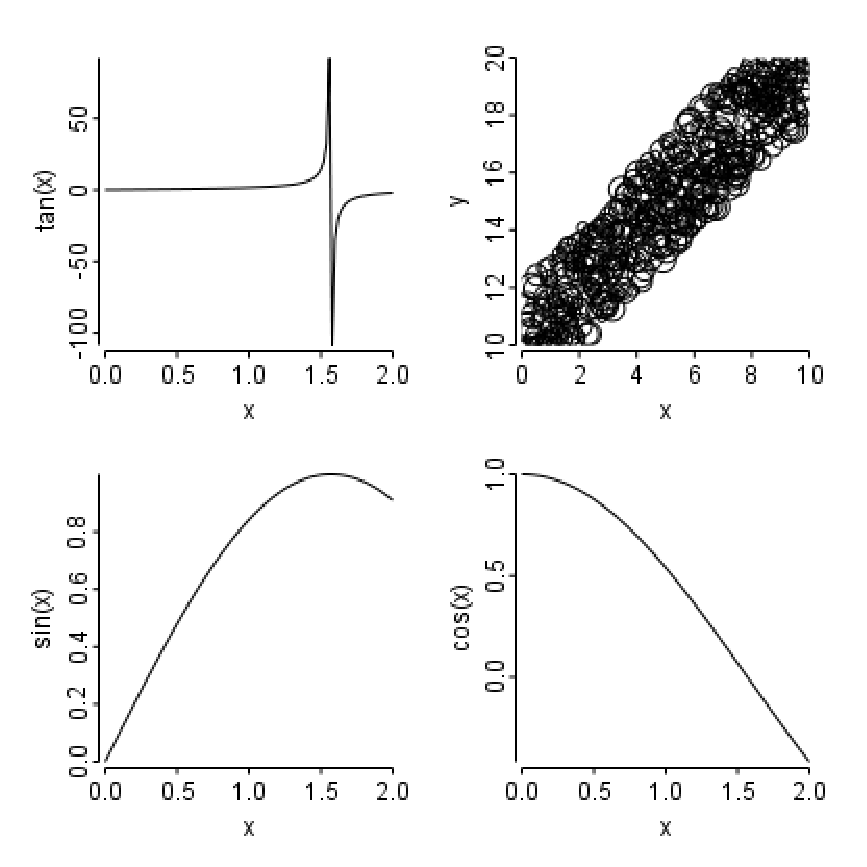
\includegraphics[width=3in,height=3in]{./test1.eps} %png
\end{frame}

\begin{frame}[fragile]{How?}
\begin{verbatim}
(defparameter *frame2*
   (as-frame (create-xlib-image-context 200 200)
   	    :background-color +white+))
(bind ((#2A((f1 f2) (f3 f4))
       (split-frame *frame2*
                    (percent 50)
                    (percent 50))))
  (defparameter *f1* f1) ; lower left   
  (defparameter *f2* f2) ; lower right  f3  f4
  (defparameter *f3* f3) ; top left     f1  f2
  (defparameter *f4* f4)); top right
\end{verbatim}
\end{frame}

\begin{frame}[fragile]{Functions to Plot}
\begin{verbatim}
(plot-function *f1* #'sin
  (interval-of 0 2)
  :x-title "x" :y-title "sin(x)")
(plot-function *f2* #'cos (interval-of 0 2)
  :x-title "x" :y-title "cos(x)")
(plot-function *f3* #'tan (interval-of 0 2)
  :x-title "x" :y-title "tan(x)")
\end{verbatim}
\end{frame}

\begin{frame}[fragile]{Things to Plot}
\small{
\begin{verbatim}
(let* ((n 500)
       (xs (num-sequence
             :from 0 :to 10 :length n))
       (ys (map 'vector
              #'(lambda (x) (+ x 8 (random 4.0)))
              xs))
       (weights
          (replicate #'(lambda () (1+ (random 10)))
                     n 'fixnum))
       (da (plot-simple *f4*
             (interval-of 0 10)
             (interval-of 10 20)
             :x-title "x" :y-title "y")))
  (draw-symbols da xs ys :weights weights))
\end{verbatim}
}
\end{frame}

\begin{frame}[fragile]{Copying existing graphics}
  And we generated the figure on the first page by:
\begin{verbatim}
(xlib-image-context-to-png
   (context *f1*)
   "/home/tony/test1.png")
\end{verbatim}
\end{frame}

\subsection{Statistical Models}
\label{sec:work:statmod}

\begin{frame}[fragile]{Linear Regression}
\small{
\begin{verbatim}
;; Worse than LispStat, wrapping LAPACK's dgelsy:
(defparameter *result1*
   (lm (list->vector-like iron)
       (list->vector-like absorbtion)))
*result*1 =>
((#<LA-SIMPLE-VECTOR-DOUBLE (2 x 1)
 -11.504913191235342
 0.23525771181009483>
  2)

 #<LA-SIMPLE-MATRIX-DOUBLE  2 x 2
 9.730392177126686e-6 -0.001513787114206932
 -0.001513787114206932 0.30357851215706255>   

 13 2)
\end{verbatim}
}
\end{frame}

\subsection{Data Manip/Mgmt}
\label{sec:work:data}

\begin{frame}[fragile]{DataFrames}
\small{
\begin{verbatim}
(defparameter *my-df-1*
  (make-instance 'dataframe-array
	 :storage #2A((1 2 3 4 5) (10 20 30 40 50))
	 :doc "This is a boring dataframe-array"
	 :case-labels (list "x" "y")
	 :var-labels (list "a" "b" "c" "d" "e")))

(xref *my-df-1* 0 0) ; API change in progress

(setf (xref *my-df-1* 0 0) -1d0)
\end{verbatim}
}
\end{frame}

\begin{frame}[fragile]{Numerical Matrices}
\small{
\begin{verbatim}
(defparameter *mat-1*
  (make-matrix 3 3
     :initial-contents #2A((2d0 3d0 -4d0)
                           (3d0 2d0 -4d0)
                           (4d0 4d0 -5d0))))

(xref *mat-1* 2 0) ; => 4d0  ; API change
(setf (xref *mat-1* 2 0) -4d0) 

(defparameter *xv*
 (make-vector 4 :type :row 
   :initial-contents '((1d0 3d0 2d0 4d0))))
\end{verbatim}
}
\end{frame}

\begin{frame}[fragile]{Macros make the above tolerable}
\begin{verbatim}
(defparameter *xv*
 (make-vector 4 :type :row 
   :initial-contents '((1d0 3d0 2d0 4d0))))

; can use defmacro for the following syntax =>

(make-row-vector *xv* '((1d0 3d0 2d0 4d0)))

; or reader macros for the following:
#mrv(*xv* '((1d0 3d0 2d0 4d0)))
\end{verbatim}
\end{frame}

\section{Discussion}

\subsection{Conclusions and Outlook}


\begin{frame}{Conclusion}

  This slowly developing research program aims to a statistical
  computing system which enables sophisticated statistical research
  which can be readily transfer to applications, is supportable.

  Related numerical/statistical projects:
  \begin{itemize}
  \item Incanter : R/LispStat/Omegahat-like system for Clojure (Lisp
    on the JVM)
  \item FEMLisp : system/workshop for finite-element analysis modeling
    using Lisp
  \item matlisp/LispLab : LAPACK-based numerical linear algebra packages
  \item GSLL : GNU Scientific Library, Lisp interface.
  \item RCL, RCLG, CLSR (embedding R within Common Lisp)
  \end{itemize}
\end{frame}

\begin{frame}{Why not use R?}
  \begin{itemize}
  \item the R programming language is incomplete and under constant
    redefinition.  Common Lisp is standardized (for many years), with
    many implementations
  \item Application delivery can be tough
  \item Without parens, Common Lisp could be R (interactive, or batch,
    or through ``compiled applications'').
  \item R is the Microsoft of statistical computing.
  \item many ``warts'' that R has, can't be fixed due to sizeable user
    populations or heavy-weight vested interests.
  \item Evolutionary development for R requires strawmen (other
    systems) upon which to use for competition.
\end{itemize}

\end{frame}

\begin{frame}{What can you do to follow up?}
  \begin{itemize}
  \item Learn common lisp, by trying it out and reading:
    \begin{itemize}
    \item \item Introduction to Common Lisp: Paul Graham's ANSI Common
      Lisp, enjoyable book with boring title, best intro to S4 classes
      around.
    \item Practical Common Lisp, by Peter Seibel
    \end{itemize}
  \item Get the packages from  http://github.com/blindglobe
  \item subscribe to the mailing list
  \end{itemize}
  The next stage of reproducible research will require computable
  statistics (code that explains itself and can be parsed to generate
  knowledge about its claims; ``XML's promise'').
\end{frame}

\begin{frame}{Thank you for listening!}
  
\end{frame}

\section{What ought to be coming}

\subsection{Theory}


\begin{frame}[fragile]{Example 1: Theory\ldots}
  \label{example1}
  Let $f(x;\theta)$ describe the likelihood of XX under the following
  assumptions.  
  \begin{enumerate}
  \item assumption-1
  \item assumption-2
  \end{enumerate}
  Then if we use the following algorithm:
  \begin{enumerate}
  \item step-1
  \item step-2
  \end{enumerate}
  then $\hat{\theta}$ should be $N(0,\hat\sigma^2)$ with the following
  characteristics\ldots
\end{frame}

\begin{frame}
  \frametitle{Can we compute, using this description?}
  Given the information at hand:
  \begin{itemize}
  \item we ought to have a framework for initial coding for the
    actual simulations (test-first!)
  \item the implementation is somewhat clear
  \item We should ask: what theorems have similar assumptions?
  \item We should ask: what theorems have similar conclusions but
    different assumptions?
  \end{itemize}
\end{frame}
\begin{frame}[fragile]{Realizing Theory}
\small{
\begin{verbatim}  
(define-theorem my-proposed-theorem
  (:theorem-type '(distribution-properties
                   frequentist likelihood))
  (:assumes '(assumption-1 assumption-2))
  (:likelihood-form
     (defun likelihood (data theta gamma)
       (exponential-family theta gamma)))
  (:compute-by
   '(progn
      (compute-start-values thetahat gammahat)
        (until (convergence)
          (setf convergence
                (or (step-1 thetahat)
                    (step-2 gammahat))))))
  (:claim (equal-distr '(thetahat gammahat) 'normal))))
\end{verbatim}
}
\end{frame}

\begin{frame}[fragile]{It would be nice to have}
\begin{verbatim}
   (theorem-veracity 'my-proposed-theorem)
\end{verbatim}
returning some indication of how well it met given computable claims,
modulo what proportion of computable claims could be tested.
\begin{itemize}
\item and have it run some illustrative simulations which suggest
  which might be problematic in real situations, and real situations
  for which there are no problems.
\item and work through some of the logic based on related claims using
  identical assumptions to confirm some of the results
\end{itemize}
\end{frame}

\begin{frame}[fragile]{and why not...?}
\begin{verbatim}
   (when (> (theorem-veracity
              'my-proposed-theorem)
            0.8)
      (make-draft-paper 'my-proposed-theorem
                        :style :JASA
                        :output-formats
                           '(LaTeX MSWord)))
\end{verbatim}
\end{frame}

\begin{frame}{Comments}
  \begin{itemize}
  \item Of course the general problem is very difficult, but one must
    start somewhere.
  \item Starting place: basic statistical proof of concepts (in
    progress ): T-Test, linear regression (LS-based, Normal-Normal
    Bayesian)
  \item Areas targetted for medium-term future: resampling methods and
    similar algorithms.
  \end{itemize}
\end{frame}

\subsection{Practice and Application}

\begin{frame}
  \frametitle{Example 2: Practice\ldots} 
  \label{example2}
  The dataset comes from a series of clinical trials, some with active
  control and others using placebo control.  We model the primary
  endpoint, ``relief'', as a binary random variable.  There is a
  random trial effect on relief as well as severity due to differences
  in recruitment and inclusion/exclusion criteria from 2 different
  trial networks.
\end{frame}

\begin{frame}
  \frametitle{Can we compute, using this description?}
  \begin{itemize}
  \item With a real such description, it is clear what some of the
    potential models might be for this dataset
  \item It should be clear how to start thinking of a data dictionary
    for this problem.
  \end{itemize}
\end{frame}

\begin{frame}[fragile]{Can we compute?}
\begin{verbatim}
(dataset-metadata paper-1
  :context 'clinical-trial 'randomized 
     'active-ctrl 'placebo-ctrl 'metaanalysis
  :variables '((relief :model-type dependent
                       :distr binary)
               (trial :model-type independent
                      :distr categorical)
               (disease-severity))
  :metadata '(incl-crit-net1 excl-crit-net1
              incl-crit-net1 excl-crit-net2
              recr-rate-net1 recr-rate-net2))
  (propose-analysis paper-1)
    ; => (list 'tables '(logistic-regression))
\end{verbatim}
\end{frame}

\subsection{Round-trip translation}


\begin{frame}{Example 3: The Round-trip\ldots} 
  \label{example3}
  The first examples describe ``ideas $\rightarrow$ code''

  Consider the last time you read someone else's implementation of a
  statistical procedure (i.e. R package code).  When you read the
  code, could you see:
  \begin{itemize}
  \item the assumptions used?
  \item the algorithm implemented?
  \item practical guidance for when you might select the algorithm
    over others? 
  \item practical guidance for when you might select the
    implementation over others? 
  \end{itemize}
  These are usually components of any reasonable journal article.
  \textit{(Q: have you actually read an R package that wasn't yours?)}
\end{frame}


\end{document}

